\def\mySecNum{3.1}
\mySection{\mySecNum~Basic insurance strategies}
%-------------- start slide -------------------------------%{{{ 1
\begin{frame}[fragile]
	Options can be
	\begin{enumerate}
		\item Used to insure long positions (floors)
		\item Used to insure short positions (caps)
		\item Written against asset positions (selling insurance)
		\item[] Covered call writing
		\item[] Covered put writing
	\end{enumerate}
\end{frame}
%-------------- end slide -------------------------------%}}}
%-------------- start slide -------------------------------%{{{ 1
\begin{frame}[fragile,t]
	\begin{center}
		Four positions
		\bigskip

		\renewcommand{\arraystretch}{1.2}
		\begin{tabular}{|c|c c|}
			\hline
			positions w.r.t. asset & put option                             & call option                       \\ \hline
			long                   & purchased (\textcolor{magenta}{floor}) & written                           \\
			short                  & written                                & purchased (\textcolor{cyan}{cap}) \\ \hline
		\end{tabular}
	\end{center}

	\bigskip
	\mySeparateLine
	\bigskip
	\begin{center}
		\begin{minipage}{0.45\textwidth}
			\centering
			Buying insurance
			\begin{align*}
				\textcolor{magenta}{floor} & = \text{buying a \textcolor{magenta}{put} option} \\
				\textcolor{cyan}{cap}      & = \text{buying a \textcolor{cyan}{call} option}
			\end{align*}
		\end{minipage}
		\begin{minipage}{0.3\textwidth}
			\centering
			Selling insurance
			\begin{align*}
				\text{Covered \textcolor{magenta}{put} writing} \\
				\text{Covered \textcolor{cyan}{call} writing}
			\end{align*}
		\end{minipage}
	\end{center}
\end{frame}
%-------------- end slide -------------------------------%}}}
%-------------- start slide -------------------------------%{{{ 1
\begin{frame}[fragile,t]
\begin{center}
	We will work under the following setup
	\bigskip
	\bigskip

	S\&S index\\
	\bigskip

	\renewcommand{\arraystretch}{1.2}
	\begin{tabular}{|c|c|}
		\hline
		index price today                                         & \$1,000  \\
    6-month interest rate                                     & 2\%      \\
		premium for 1000-strike 6-month \textcolor{magenta}{call} & \$93.809 \\
		premium for 1000-strike 6-month \textcolor{cyan}{put}     & \$74.201 \\ \hline
	\end{tabular}

\end{center}

\end{frame}
%-------------- end slide -------------------------------%}}}
%-------------- start slide -------------------------------%{{{ 1
\begin{frame}[fragile]
	\frametitle{Insuring a long position \\ -- \textcolor{magenta}{Floors}}

	\begin{center}
		\renewcommand{\arraystretch}{1.2}
		\begin{tabular}{|c|c|}
			owning a home      & owning a stock index                      \\
			insuring the house & buying a put (\textcolor{magenta}{floor}) \\
		\end{tabular}
		\bigskip
		\bigskip

		Goal: to insure against a fall in the price of the underlying asset.
	\end{center}

\end{frame}
%-------------- end slide -------------------------------%}}}
%-------------- start slide -------------------------------%{{{ 1
\begin{frame}[fragile]
	\begin{myexample}
		Under the following scenario, compute the combined profit of \underline{insuring a long
		position via \textcolor{cyan}{buying a put}} for the following S\&R index.
	\begin{center}
		\renewcommand{\arraystretch}{1.2}
		\begin{tabular}{|c|c|}
			\hline
			index price today                                     & \$1,000  \\
			6-month interest rate                                 & 2\%      \\
			% premium for 1000-strike 6-month call & \$93.809 \\ \hline
			premium for 1000-strike 6-month \textcolor{cyan}{put} & \$74.201 \\ \hline
			index price at expiration                             & \$900    \\ \hline
		\end{tabular}
	\end{center}
	\end{myexample}
	\vfill
	\pause
	\begin{mysol}
		\begin{align*}
			\underbrace{\$900 - \$1,000 \times 1.02}_{\text{profit on S\&R index}} +
			\underbrace{\$1,000-\$900 -\$74.201 \times 1.02}_{\text{profit on put}} = -\$95.68.
		\end{align*}
		\myEnd
	\end{mysol}
\end{frame}
%-------------- end slide -------------------------------%}}}
%-------------- start slide -------------------------------%{{{ 1
\begin{frame}[fragile,t]
	\begin{center}
		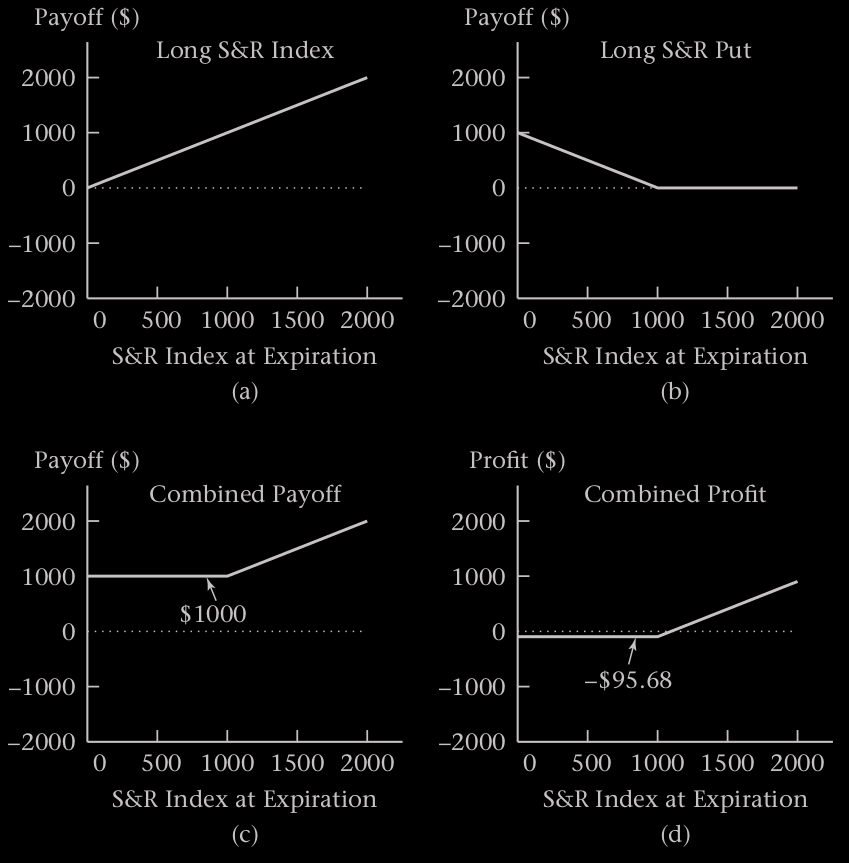
\includegraphics[scale=0.25]{figs/Figure-3-1.png}
	\end{center}
\end{frame}
%-------------- end slide -------------------------------%}}}
%-------------- start slide -------------------------------%{{{ 1
\begin{frame}[fragile]
\begin{center}
	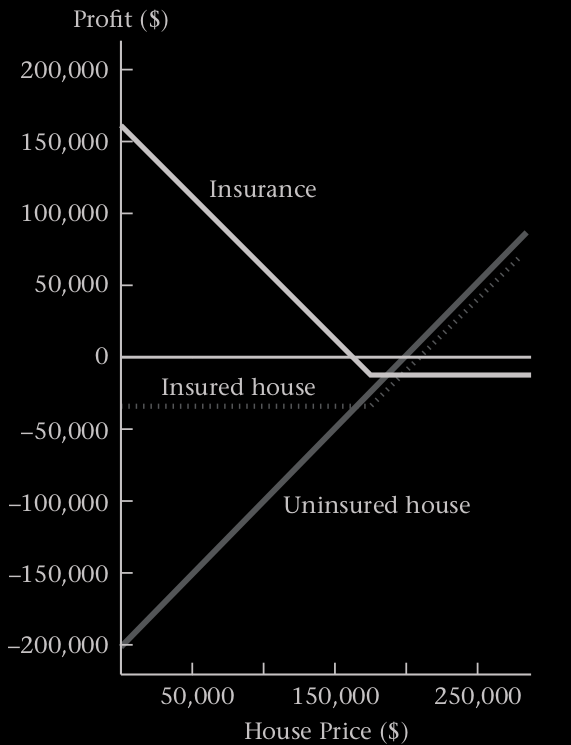
\includegraphics[scale=0.2]{figs/Figure-3-2.png}
\end{center}
\end{frame}
%-------------- end slide -------------------------------%}}}
%-------------- start slide -------------------------------%{{{ 1
\begin{frame}[fragile,t]
	\frametitle{Insuring a short position \\ -- \textcolor{magenta}{Caps}}

If we have a short position in the S\&R index, we experience a loss when the index rises.
\bigskip

We can insure a short position by \textcolor{cyan}{purchasing a call option (cap)} to protect against a
higher price of repurchasing the index.

\end{frame}
%-------------- end slide -------------------------------%}}}
%-------------- start slide -------------------------------%{{{ 1
\begin{frame}[fragile]
	\begin{myexample}
		Under the following scenario, compute the combined profit for \underline{insuring a short
		position via \textcolor{magenta}{buying a call}} of the following S\&R index.

		\begin{center}
			\renewcommand{\arraystretch}{1.2}
			\begin{tabular}{|c|c|}
				\hline
				index price today                                         & \$1,000  \\
				6-month interest rate                                     & 2\%      \\
				premium for 1000-strike 6-month \textcolor{magenta}{call} & \$93.809 \\ \hline
				% premium for 1000-strike 6-month put & \$74.201 \\ \hline
				index price at expiration                                 & \$1,100  \\ \hline
			\end{tabular}
		\end{center}
	\end{myexample}
	\vfill
	\pause
	\begin{mysol}
		\begin{align*}
			\underbrace{\$1,000 \times 1.02}_{\text{future value of short S\&R index}} - \: \:
			\underbrace{\$93.809 \times 1.02}_{\text{FV of premium for call}} - \:\:
			\underbrace{\$1,000}_{\text{exercise the call option}}
			= -\$75.685.
		\end{align*}
		\myEnd
	\end{mysol}
\end{frame}
%-------------- end slide -------------------------------%}}}
%-------------- start slide -------------------------------%{{{ 1
\begin{frame}[fragile]
	\begin{center}
		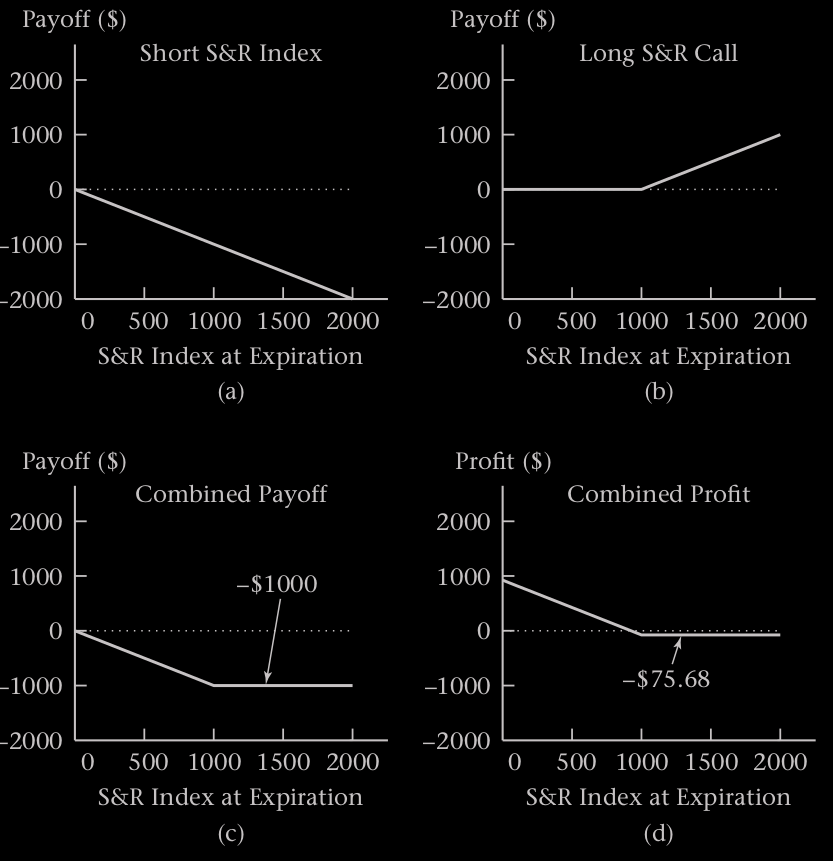
\includegraphics[scale=0.25]{figs/Figure-3-3.png}
	\end{center}
\end{frame}
%-------------- end slide -------------------------------%}}}
%-------------- start slide -------------------------------%{{{ 1
\begin{frame}[fragile,t]
	\frametitle{Selling insurance}
	\centering

	For every insurance buyer there must be an insurance seller

	\pause
	\bigskip
	\mySeparateLine
	\bigskip

	Strategies used to sell insurance
	\pause
	\bigskip

	\begin{itemize}
		\item \textcolor{magenta}{Covered writing} (\textcolor{magenta}{option overwriting} or
			\textcolor{magenta}{selling a covered call}) is writing an option when there is a corresponding long position in the
			underlying asset.

			\bigskip
		\item \textcolor{magenta}{Naked writing} is writing an option when the writer does not have a
			position in the asset.
	\end{itemize}
\end{frame}
%-------------- end slide -------------------------------%}}}
%-------------- start slide -------------------------------%{{{ 1
\begin{frame}[fragile]
\begin{center}

	\begin{minipage}{0.6\textwidth}
		\centering

		\textcolor{magenta}{Covered call writing}
		\bigskip

		Long position of the asset  + Sell a \textcolor{magenta}{call} option
	\end{minipage}
	$ \quad  \sim$
	\begin{minipage}{0.3\textwidth}
		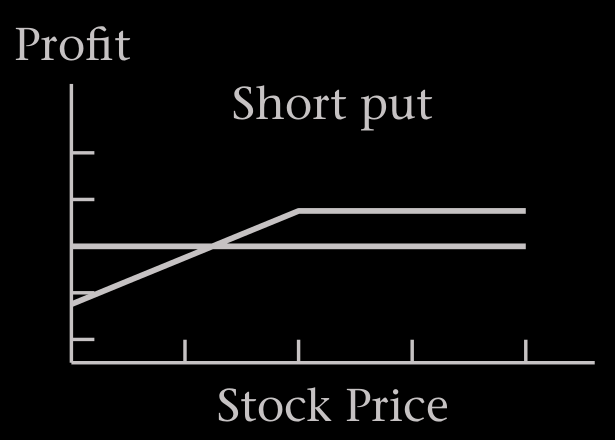
\includegraphics[scale=0.15]{figs/Short-put.png}
	\end{minipage}

	\mySeparateLine
	\bigskip

	\begin{minipage}{0.6\textwidth}
		\centering

		\textcolor{cyan}{Covered put writing}
		\bigskip

		Short position of the asset  + Sell a \textcolor{cyan}{put} option
	\end{minipage}
	$ \quad  \sim$
	\begin{minipage}{0.3\textwidth}
		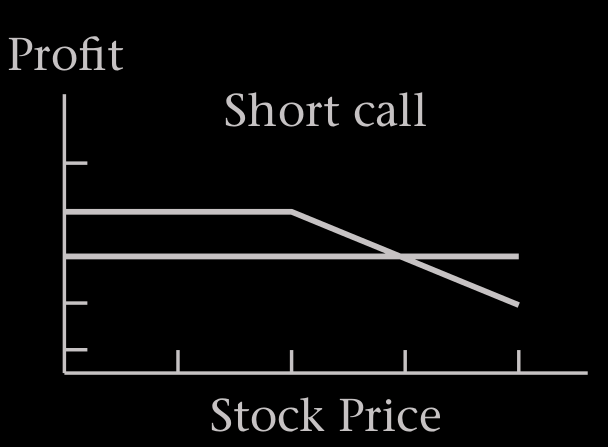
\includegraphics[scale=0.15]{figs/Short-call.png}
	\end{minipage}

\end{center}
\end{frame}
%-------------- end slide -------------------------------%}}}
%-------------- start slide -------------------------------%{{{ 1
\begin{frame}[fragile,t]
	\frametitle{Covered call writing}

	\begin{myexample}
		Under the following scenario, compute the combined profit for \underline{writing a
		\textcolor{magenta}{covered call}}
		for S\&R index.
		\begin{center}
			\renewcommand{\arraystretch}{1.2}
			\begin{tabular}{|c|c|}
				\hline
				index price today                                         & \$1,000  \\
				6-month interest rate                                     & 2\%      \\
				premium for 1000-strike 6-month \textcolor{magenta}{call} & \$93.809 \\ \hline
				% premium for 1000-strike 6-month \textcolor{cyan}{put} & \$74.201 \\ \hline
				index price at expiration                                 & \$1,100  \\ \hline
			\end{tabular}
		\end{center}
	\end{myexample}
	\vfill
	\pause
	\begin{mysol}
		\begin{align*}
			\underbrace{\$1,100 - \$1,000 \times 1.02}_{\text{profit on S\&R index}} +
			\underbrace{\$1,000-\$1,100 +\$93.809 \times 1.02}_{\text{profit on written call}} = \$75.68.
		\end{align*}
		\myEnd
	\end{mysol}
\end{frame}
%-------------- end slide -------------------------------%}}}
%-------------- start slide -------------------------------%{{{ 1
\begin{frame}[fragile]
	\begin{center}
		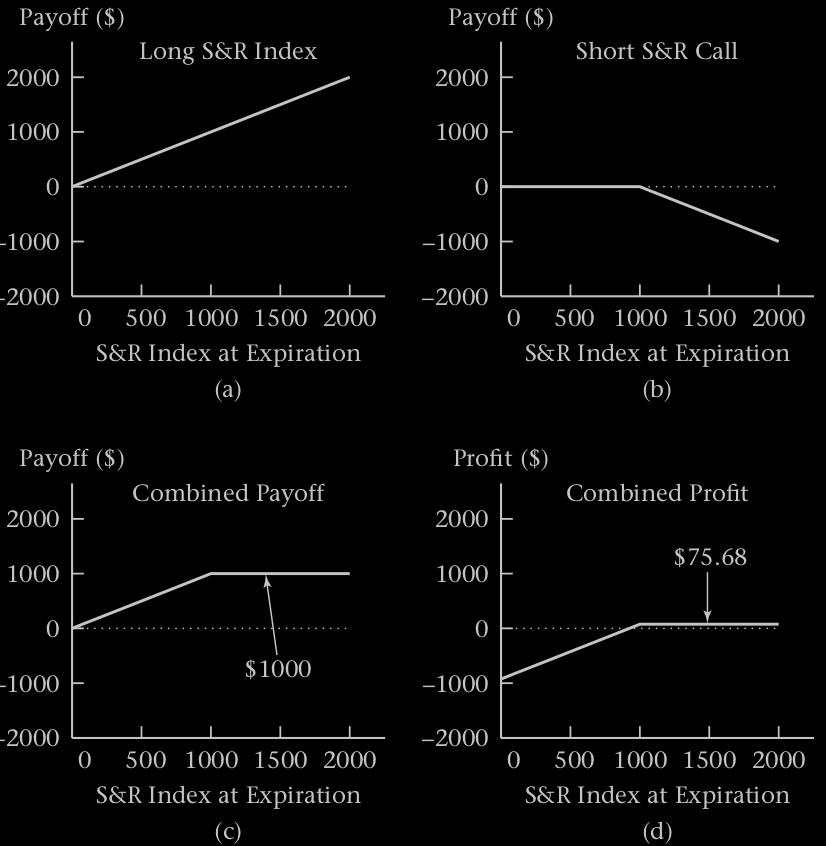
\includegraphics[scale=0.25]{figs/Figure-3-4.png}
	\end{center}
\end{frame}
%-------------- end slide -------------------------------%}}}
%-------------- start slide -------------------------------%{{{ 1
\begin{frame}[fragile,t]
	\frametitle{Covered put writing}
	\begin{myexample}
		Under the following scenario, compute the combined profit for \underline{writing a
		\textcolor{cyan}{covered put}}
		for S\&R index.
		\begin{center}
			\renewcommand{\arraystretch}{1.2}
			\begin{tabular}{|c|c|}
				\hline
				index price today                                     & \$1,000  \\
				6-month interest rate                                 & 2\%      \\
				% premium for 1000-strike 6-month \textcolor{magenta}{call} & \$93.809 \\ \hline
				premium for 1000-strike 6-month \textcolor{cyan}{put} & \$74.201 \\ \hline
				index price at expiration                             & \$900  \\ \hline
			\end{tabular}
		\end{center}
	\end{myexample}
	\vfill
	\pause
	\begin{mysol}
		\begin{align*}
			\underbrace{\$1,000 \times 1.02 - \$900}_{\text{profit on selling S\&R index}} +
			\underbrace{\$900-\$1,000 +\$74.201 \times 1.02}_{\text{profit on written put}} = \$95.685.
		\end{align*}
		\myEnd
	\end{mysol}
\end{frame}
%-------------- end slide -------------------------------%}}}
%-------------- start slide -------------------------------%{{{ 1
\begin{frame}[fragile]
	\begin{center}
		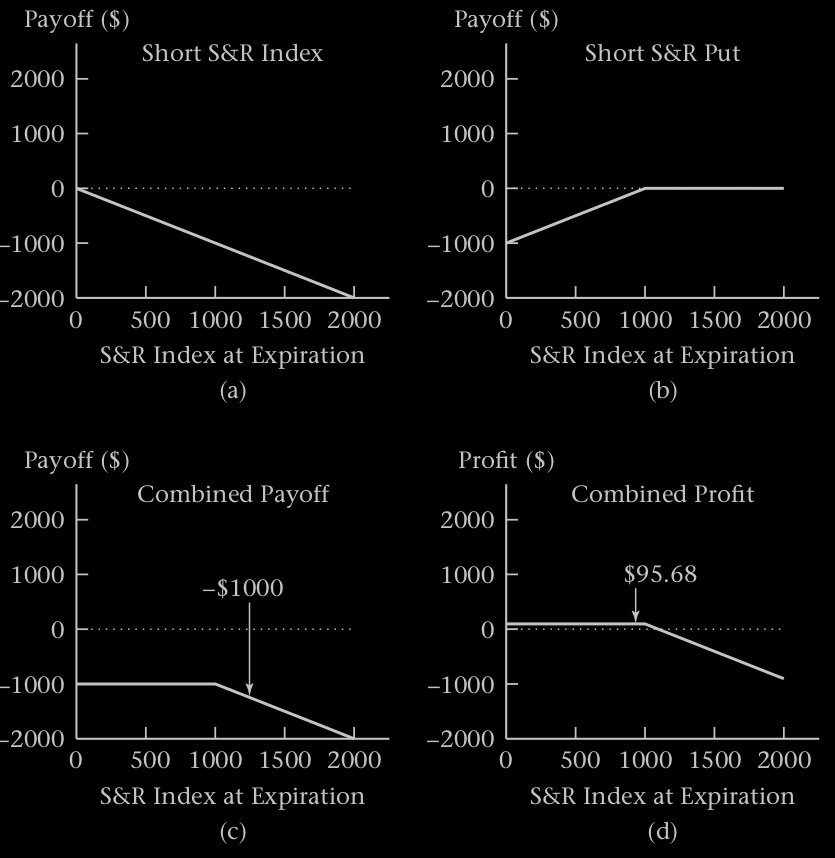
\includegraphics[scale=0.25]{figs/Figure-3-5.png}
	\end{center}
\end{frame}
%-------------- end slide -------------------------------%}}}
